\documentclass{article}
\usepackage{graphicx}
\usepackage[margin=1.5cm]{geometry}
\usepackage{amsmath}
\usepackage{fancyvrb}
\usepackage{url}

\begin{document}

\title{Synopsis - Week 9 Integrated Project: Probing Fixed IC Counters with Oscilloscope, DC Power Supply, Breadboard, and Digital Voltmeter}
\author{Prof. Jordan C. Hanson}

\maketitle

\section{Reading the Specification Sheet of IC Counter}

Today we will be working with the Texas Instruments SN54HC4040 component.  This is a 16-pin, 12-bit, asynchronous counter.  The specification sheet is posted to the course Moodle page, under Week 9.  Note the specification includes the functional block diagram (Fig. \ref{fig:count1}, left).  Note that there are 12 flip-flops, making the SN54HC4040 a 12-bit counter.  The gate logic before the pin-1 flip-flop involves the clear (CLR) and clock (CLK) signals.  The clock is inverted, so a high-to-low transition starts the count.  The CLR signal is split and then passed into an OR (after being inverted and un-inverted).  The CLR is connected to all flip-flop reset inputs, so a HIGH on CLR resets the counter.

\begin{figure}[ht]
\centering
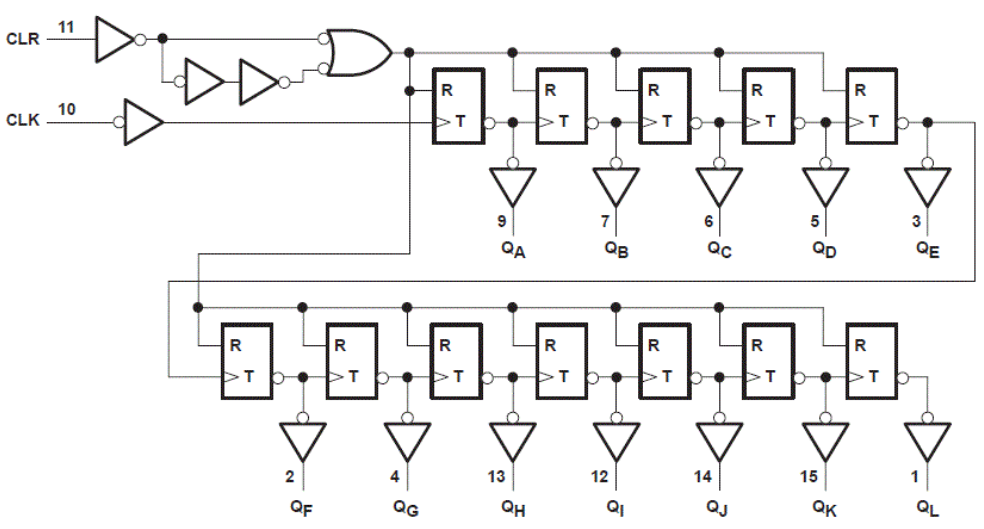
\includegraphics[width=0.45\textwidth]{counter_1.png} \hspace{1cm}
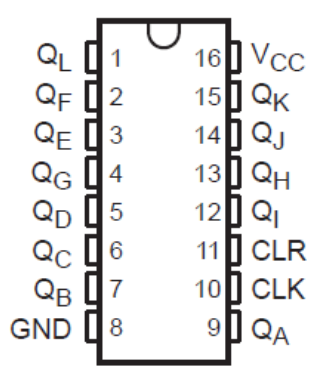
\includegraphics[width=0.15\textwidth]{counter_2.png}
\caption{\label{fig:count1} (Left) The functional block diagram of the SN54HC4040. (Right) The pinout for the SN54HC4040 16-pin DIP.  Note the locations of $V_{\rm CC}$, CLR, CLK, and GND.}
\end{figure}

\noindent
Using the Table of Contents and tables within the specification sheet, answer the following questions.
\begin{itemize}
\item What is the maximum range for $V_{\rm CC}$, the supply voltage? \vspace{0.25cm}
\item If the supply voltage is 3.3V to 5V, what is the minimum input HIGH voltage, $V_{\rm IH}$? \vspace{0.25cm}
\item If the supply voltage is 3.3V to 5V, what is the maximum input LOW voltage, $V_{\rm IL}$? \vspace{0.25cm}
\item What is the maximum clock frequency, $f_{\rm CLK}$, of the SN54HC4040 if $V_{\rm CC} = 2$V? \vspace{0.25cm}
\end{itemize}

\section{Breadboard Setup, Connecting the IC Counter}

Make sure that your lap table is powered, and that the DC power supply is connected.  Switch on the power supply, and use the digital voltmeter to check that the voltage between the red and black (GND) terminals is 3.3 V.  Use the red and black banana-plug cables to route power down to your breadboard.  Use the red breadboard post for $V_{\rm CC}$, and the black post for GND.  Use the DVM to check that the voltage between the posts is still 3.3V.  Now turn off the DC power supply.  Unscrew the red post cap until you find a hole through the post.  Do the same for the black post.  Slide jumper wires into these holes, and then screw the post down to hold the jumpers in place.  Orient the posts away from you on the table.  Note in Fig. \ref{fig:count1} (right) the pinout of the DIP package for the IC counter contains a notch near pins 1 and 16.  Straddle the counter across the center divide of the breadboard such that pins 1 and 16 are oriented away from you.  The counter should be within range of the jumpers so that the hot jumper can bring $V_{\rm CC}$ to pin 16, and the GND jumper can bring GND to pin 8.
 
\begin{figure}
\centering
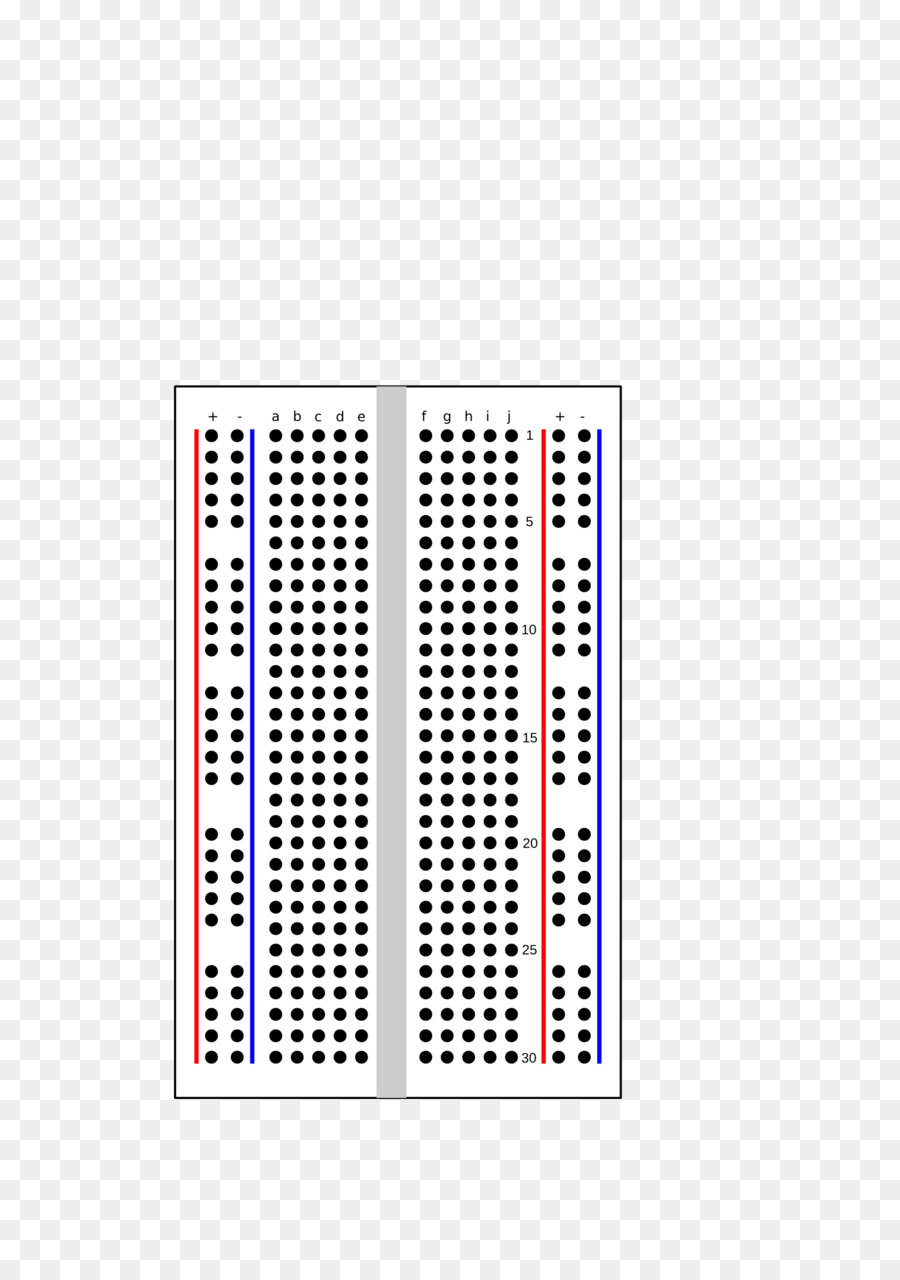
\includegraphics[width=0.20\textwidth,trim=5cm 6cm 9cm 13cm,clip=true]{breadboard.jpg} \hspace{0.5cm}
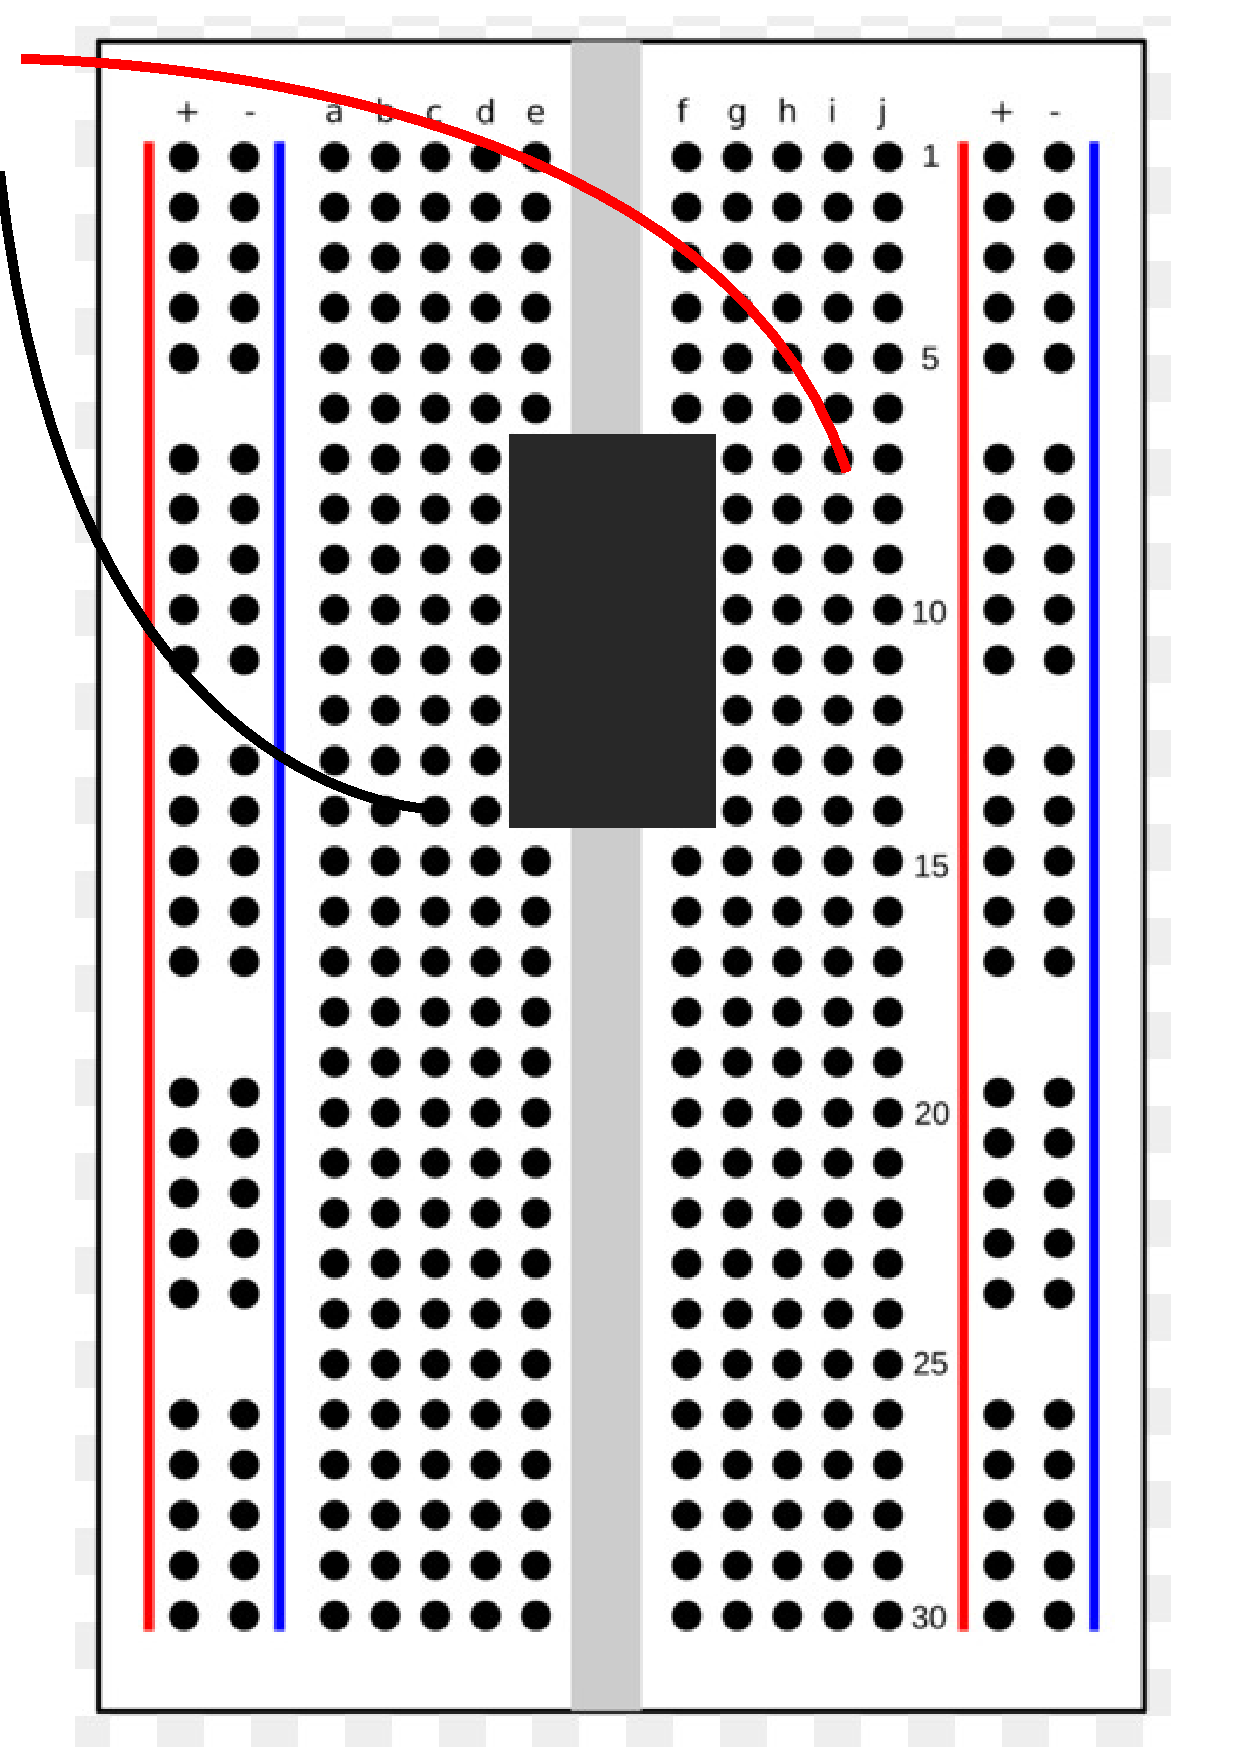
\includegraphics[width=0.21\textwidth]{breadboard_power.pdf}
\caption{\label{fig:count2} (Left) The basic breadboard layout.  The rows of five pins are connected, but the connection does not persist across the center divide.  Outer columns of five pins are also connected. (Right) Place the IC counter across the divide, and connect $V_{\rm CC}$ to pin 1 and GND to pin 8.}
\end{figure}

\section{Generating a Clock Signal with the Oscilloscope Signal Generator}

On the oscilloscope, there is a built-in signal generator.  The button to activate it is named ``wave gen.''  Press it to open the signal generator menu.  If a message appears indicating the wave generator is not available, we will use a separate signal generator.  Use the controls to create a square wave.  Use the Timing Characteristics table in the SN54HC4040 spec sheet to determine the maximum clock frequency.  Choose the highest frequency that (a) is producable by the signal generator, and (b) below the maximum clock frequency for the SN54HC4040.  We recommend the leading digit of the chosen clock frequency be a power of 2, but this is not mandatory if a higher frequency is desired.  Connect a BNC coaxial cable from the signal output to the channel 1 scope input.  Use the spec sheet to determine what CLK amplitude is appropriate.  \textbf{Please ensure that the minimum voltage of CLK signal is 0V.}  Adjust the scope trigger settings such that the scope displays the CLK signal on channel 1.

\section{Wiring the IC Counter with CLK, Holding CLR Signal LOW}

Our next job is to provide the CLK signal to the IC counter, and to ensure that the CLR signal is LOW.  In the lab, there are special coaxial cables with BNC connectors on one side, and red/black leads on the other side.  Connect the CLK signal to the BNC side, and use the leads with jumpers to deliver the CLK signal to the board.  Connect the black CLK lead to GND with a jumper, connect the red CLK lead to pin 10, and jump GND to CLR on pin 11 (Fig. \ref{fig:count3}, left).

\begin{figure}[hb]
\centering
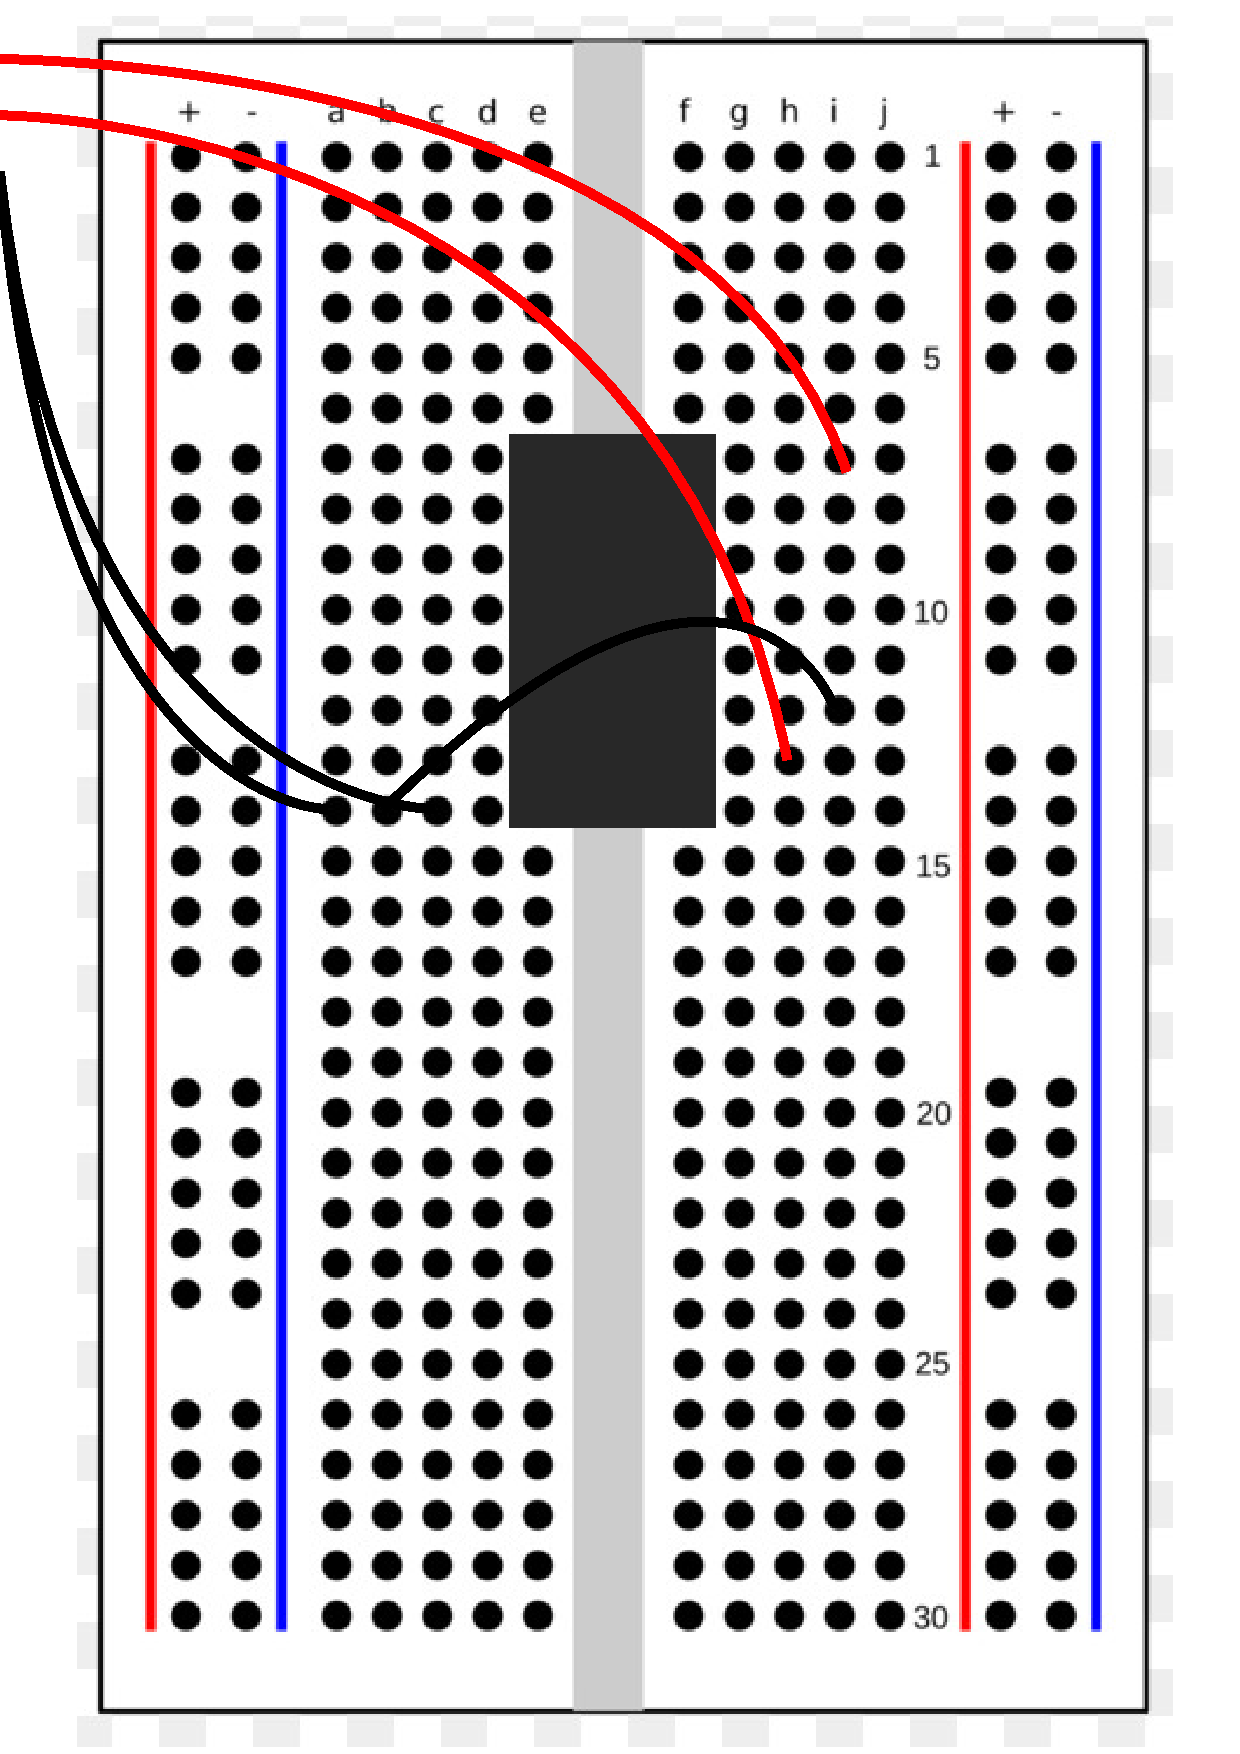
\includegraphics[width=0.21\textwidth]{breadboard_power_clk_reset.pdf}
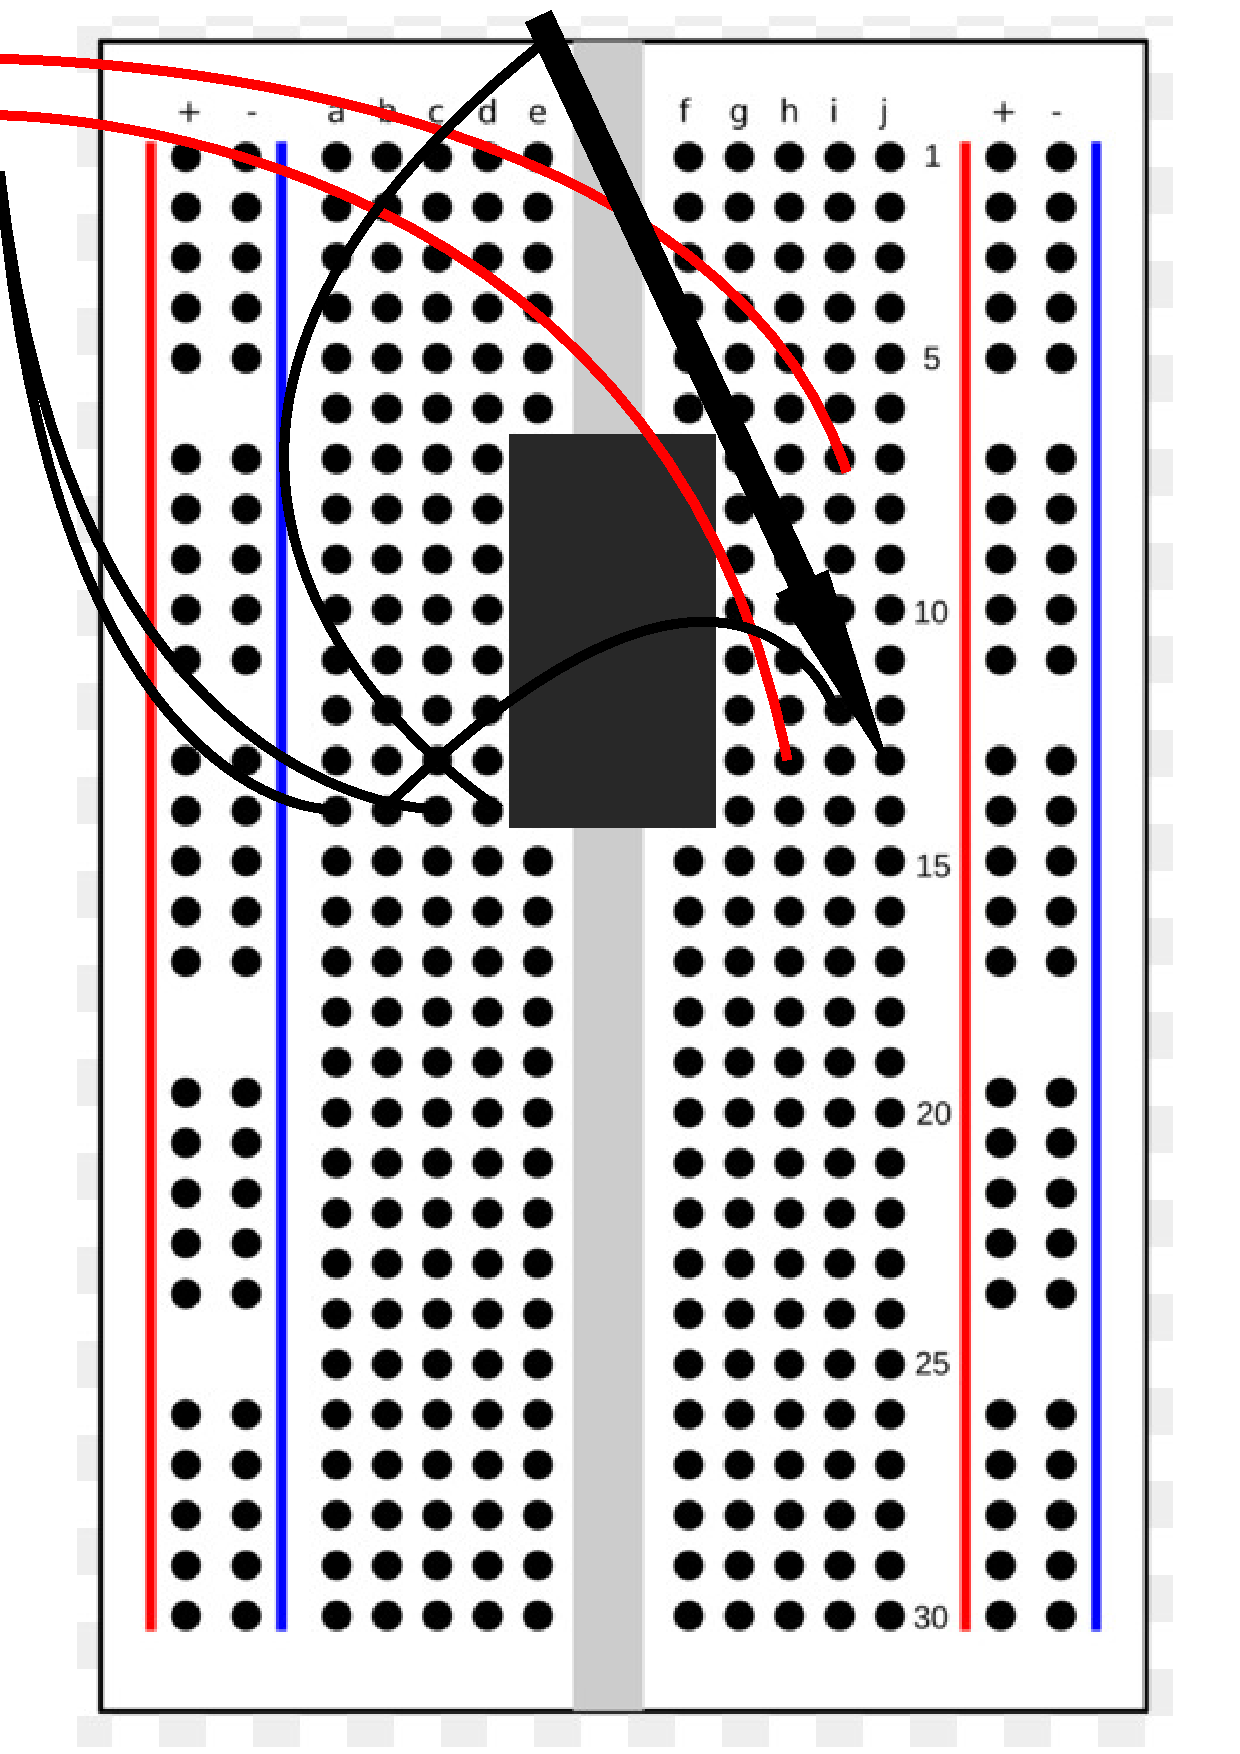
\includegraphics[width=0.21\textwidth]{breadboard_power_clk_reset_probe.pdf}
\caption{\label{fig:count3} (Left) The CLK signal is connected to pin 10 and GND.  The CLR signal is held LOW by connecting it to GND. (Right) The probe is connected to GND, and the tip passes the signal to the scope.}
\end{figure}

\section{Probing IC Counter Channels with Scope Probe}

Connect the scope probe BNC connector to scope channel 1.  Connect the probe to GND using the GND clip and a jumper.  Use the probe tip to probe the CLK signal on the breadboard (Fig. \ref{fig:count3}, right).

\begin{itemize}
\item Adjust the scope trigger settings to trigger on the probe signal.
\item Locate the Measurement section of the scope panel.  Press the Measurement button to bring up a menu at the bottom of the screen.
\item Add a measurement, and choose Frequency as the measurement.  Is the measured frequency the same as the chosen CLK frequency?
\item Consult the spec sheet to determine which pin corresponds to the LSB in the count.  Probe that pin and record its frequency in the table below.
\item Repeat the prior step, adjusting trigger and channel 1 controls as necessary to obtain frequency measurements.
\item Do you identify the correct pattern in the frequency measurements?  Explain why below.
\end{itemize}

\begin{table}
\centering
\begin{tabular}{| c | c | c |}
\hline
Pin & Frequency [MHz] & Frequency [MHz] / $f_{\rm CLK}$ [MHz] \\ \hline
9 & & \\ \hline
7 & & \\ \hline
6 & & \\ \hline
5 & & \\ \hline
3 & & \\ \hline
2 & & \\ \hline
4 & & \\ \hline
13 & & \\ \hline
12 & & \\ \hline
14 & & \\ \hline
15 & & \\ \hline
\end{tabular}
\caption{\label{tab:data} Fill in your frequency measurments in the second column, and divide them by $f_{\rm CLK}$ in the third column.}
\end{table}

\end{document}
